\subsection{Viscous standing waves}%Re=250,2500.

Computing the dissipation due to wave-breaking remains a challenging problem in the computational fluid mechanics context. In order to analyze the solution with PFEM-2 of two-phase viscous incompressible flows, the evolution of a viscous standing wave has been chosen. This is a classical problem in the scientific literature for which an approximate analytical solution is available for small amplitude perturbations\cite{Lighthill01} and it is of practical interest since it is related to the propagation of gravity waves.

The chosen standing wave configuration consists in a rectangular tank with length $L$ and a water filling height of $H = L/2$. This setup is taken from \cite{Colagrossi12}, and in the Figure \ref{fg:standing-wave-config} a sketch of this configuration is displayed. The wave length is $\lambda = L$, $k$ is the corresponding wave number (i.e. $k = 2\pi/\lambda$), $A$ is the wave amplitude and denotes the ratio $\epsilon=2A/H$.

\begin{figure}[H]
  \begin{center}
      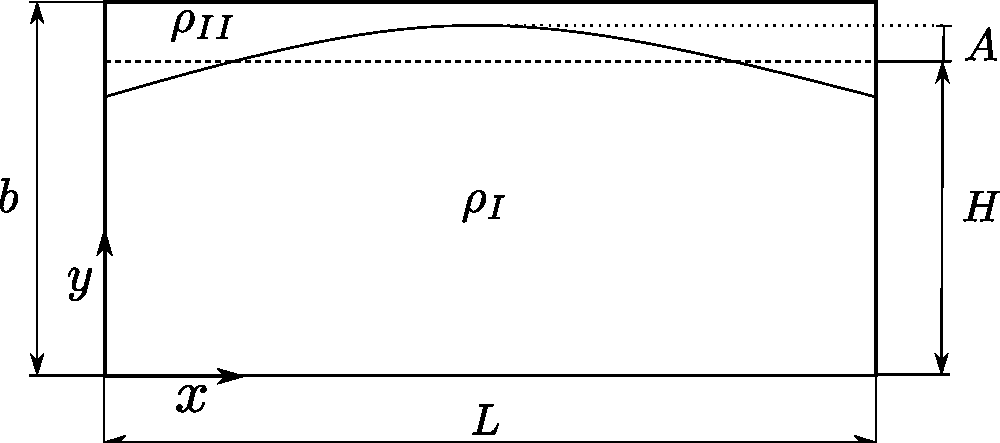
\includegraphics[width=.7\columnwidth]{images/standing_wave.pdf}
  \end{center}
  \caption{\label{fg:standing-wave-config} Configuration scheme of standing wave case. Initial condition is represented by dotted lines. In continuous line is presented an intermediate state where the maximum amplitude $A$ is reached.}
\end{figure}

If the fluid is viscous, the dissipation due to the solid boundary layers is neglected, small-amplitude waves (i.e small $\epsilon$) and small wave steepness (i.e $2A/\lambda \ll 0.1$) are used; an approximate analytical solution of the standing wave evolution can be obtained through the linearization of Navier-Stokes equations for traveling waves:
\begin{align}
 \varphi(x,y,t) & = \varphi_0(x,y)\cos(\omega t) \\
 \varphi_0(x,y) & =-\epsilon\frac{Hg}{2\omega}\frac{\cosh\left[k(y+H)\right]}{\cosh(kH)}\cos(kx)
\end{align}

where the circular frequency $\omega$ is given by the dispersion relation of gravity waves, that is, $\omega^2 = g k \tanh(kH)$ where $g$ is the acceleration of gravity. At time $t = 0$ the free surface is horizontal while the initial fluid velocity is given by $\varphi_0$.

It can be demonstrated that the approximate solution is well posed only for $Re\gg1$ and for $Re^{-1}\ll k \ll Re^{2/3}$, where $Re=H\sqrt{gH}/\nu$ is the Reynolds number for this problem. From that solution, it is possible to obtain the formula that gives the approximate decay of the kinetic energy\cite{Lighthill01}:

\begin{equation}
 \varepsilon_K(t) = \epsilon^2g\frac{\lambda H^2}{32}e^{-4\nu k^2t}\left[1+\cos(2\omega t)\right]
 \label{kin-eq}
\end{equation}

The kinetic attenuation is governed by the coefficient of the exponential $\beta_l = 4\nu k^2$, which depends on the wave number and on the kinematic viscosity $\nu = \mu/\rho_{I}$. Lately work\cite{Antuono13} has demonstrated that generally, the Equation \ref{kin-eq} overestimates the dissipations, especially when the Reynolds number is not very large. Then an improved damping rate is proposed in that paper $\beta = 4\nu k^2 -  2\sqrt{2}k^{11/4}Re^{-3/2}+O(Re^{-2})$, which is next used for comparisons.

To accomplish the linear solution hypothesis, the PFEM-2 simulations have been implemented by using a free-slip condition for the velocity and a Neumann condition for the pressure along each boundary of the tank. Also, the parameters $L=2$, $A=0.05$ and $g=1$ have been selected.

Several Reynolds number ($Re=25,50,250,2500$) have been selected to compare with the approximate analytic dissipation. Problems were solved into a grid with $H/\Delta x=100$ and varying $\Delta t$ in order to solve using a Fourier number $Fo=\frac{\nu\Delta t}{\Delta x^2}$ with a local maximum of $Fo_{max}\approx10-50$. Figure \ref{fg:sw-energy} shows the comparison between the expected dissipation (which includes the improving damping rate) and numerical results with PFEM-2. Large Fourier numbers were used in order to reduce the computation times required to complete the simulations and to show the accuracy of the method working not only with large CFL numbers, even with large diffusion rate.

  \begin{figure}[h]
  \centering
    \subfloat[]{
	  \label{fg:sw-energy-25}
	  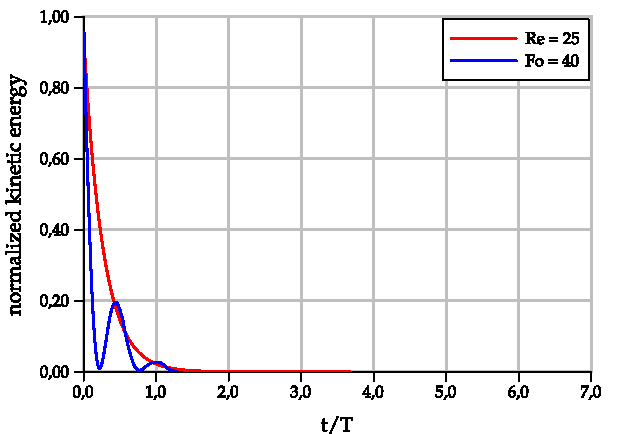
\includegraphics[width=.49\columnwidth]{images/sw_25.pdf}
    }
    \subfloat[]{
	  \label{fg:sw-energy-50}
	  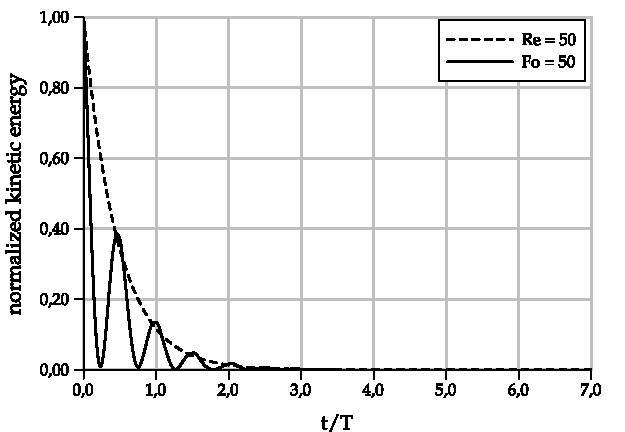
\includegraphics[width=.49\columnwidth]{images/sw_50.pdf}
    } \\
    \subfloat[]{
	  \label{fg:sw-energy-250}
	  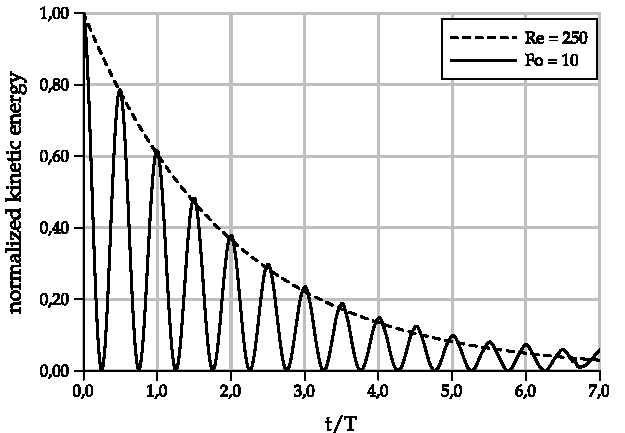
\includegraphics[width=.49\columnwidth]{images/sw_250.pdf}
    }
    \subfloat[]{
	  \label{fg:sw-energy-2500}
	  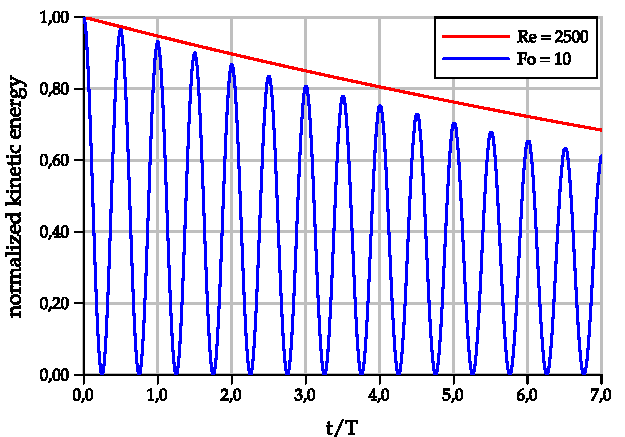
\includegraphics[width=.49\columnwidth]{images/sw_2500.pdf}
    }
   \caption{Kinetic Energy decay for standing wave problem with different Reynolds numbers. Dotted lines are approximate analytical solutions for total energy and filled lines are the kinetic energy calculated with PFEM-2. Reynolds numbers analyzed: $Re=25,50,250,2500$ in Figures \ref{fg:sw-energy-25},\ref{fg:sw-energy-50},\ref{fg:sw-energy-250},\ref{fg:sw-energy-2500} respectively. Legend in each figure indicates the maximum Fourier number used in each numerical simulation.}
   \label{fg:sw-energy}
\end{figure}
% \afterpage{\clearpage}
